%!TEX root = ../tesi.tex

\chapter{Il Progetto SF-Remote-Connection}
\label{ch:sfremoteconnection}

Vengono ora presentati i moduli software realizzati nel corso dello sviluppo del progetto di tesi.
Per meglio comprendere gli aspetti di sviluppo legati al progetto \`e importante tener conto degli obbiettivi di progetto esposti al paragrafo \ref{sec:obbiettivo} e della descrizione dei meccanismi di gestione dati interni del framework, descritti nel capitolo \ref{ch:gestionedati}.

Nella sezione \ref{sec:moduli} del capitolo viene fornita innanzitutto una suddivisione e una descrizione dei moduli, nella sezione \ref{sec:dataset_sost} viene descritto il meccanismo dei Dataset sostitutivi
e nella \ref{sec:rete} l'infrastruttura di ret e il protocollo di comunicazione.
Infine \`e presente una panoramica sui package java e le principali classi di ognuno di essi nella sezione \ref{sec:sfrc_packages}.

\`E giusto sottolineare che l'obbiettivo principale \`e stato la produzione di librerie e tool per lo sviluppo di applicazioni, focalizzandosi sull'estendibilit\`a e il riutilizzo del codice. Non a caso sono infatti presenti alcuni riferimenti di appendice ad alcuni design pattern particolarmente significativi nella produzione di questo tipo di softwaree e che sono utilizzati sia dal framework che dai moduli stessi.

Per il processo di sviluppo \`e stata di fondamentale importanza la produzione parallela di una serie di test, presentati nel capitolo \ref{ch:testerisultati}. Infatti la progettazione e la realizzazione dei moduli e dei meccanismi presentati in questo capitolo non \`e stata svolta in maniera distinta, ma si \`e trattato di un processo iterativo in cui i test hanno svolto pi\`u di una volta un ruolo di guida nel refactoring del codice.

Si rimanda all'appendice \ref{a:notesoftware} per informazioni sul codice sorgente relativo al progetto e per informazioni sulle versioni delle librerie utilizzate.

% TODO: cambiare titolo?
\section{Moduli} 
\label{sec:moduli}
La libreria di classi realizzata pu\`o essere suddivisa in quattro macro-moduli suddivisi in base alle finalit\`a e alle funzionalit\`a.
Di seguito viene data una descrizione degli stessi in questo ordine:
\begin{enumerate}
	\item \textbf{Base Communication}
	\item \textbf{RemoteDataCenter Tool}
	\item \textbf{Client}
	\item \textbf{Server}
\end{enumerate}

% TODO: 
%	inserire un'immagine di come i moduli funzionino su vari livelli
%	verificare i nomi e le appartenenze dei package

\subsection{Base Communication}
\label{sub:basecommodule}
Questo modulo riunisce le classi che consentono la creazione e la gestione di connessioni TCP/IP tra applicazioni client/server. Ne fa parte anche la classe di utilit\`a \texttt{GenericCommunicator} che oltre a consentire la gestione della connessione assegnatagli la utilizza per fornire funzionalit\`a di lettura e scrittura di messaggi testuali attraverso il canale aperto.

Il modulo \`e composto dai package \texttt{sfrc.base.communication} e \\\texttt{sfrc.base.communication.sfutil}.

\subsection{RemoteDataCenter Tool}
\label{sub:remotedatacentertoolmodule}

\begin{figure}[t]
\begin{center}
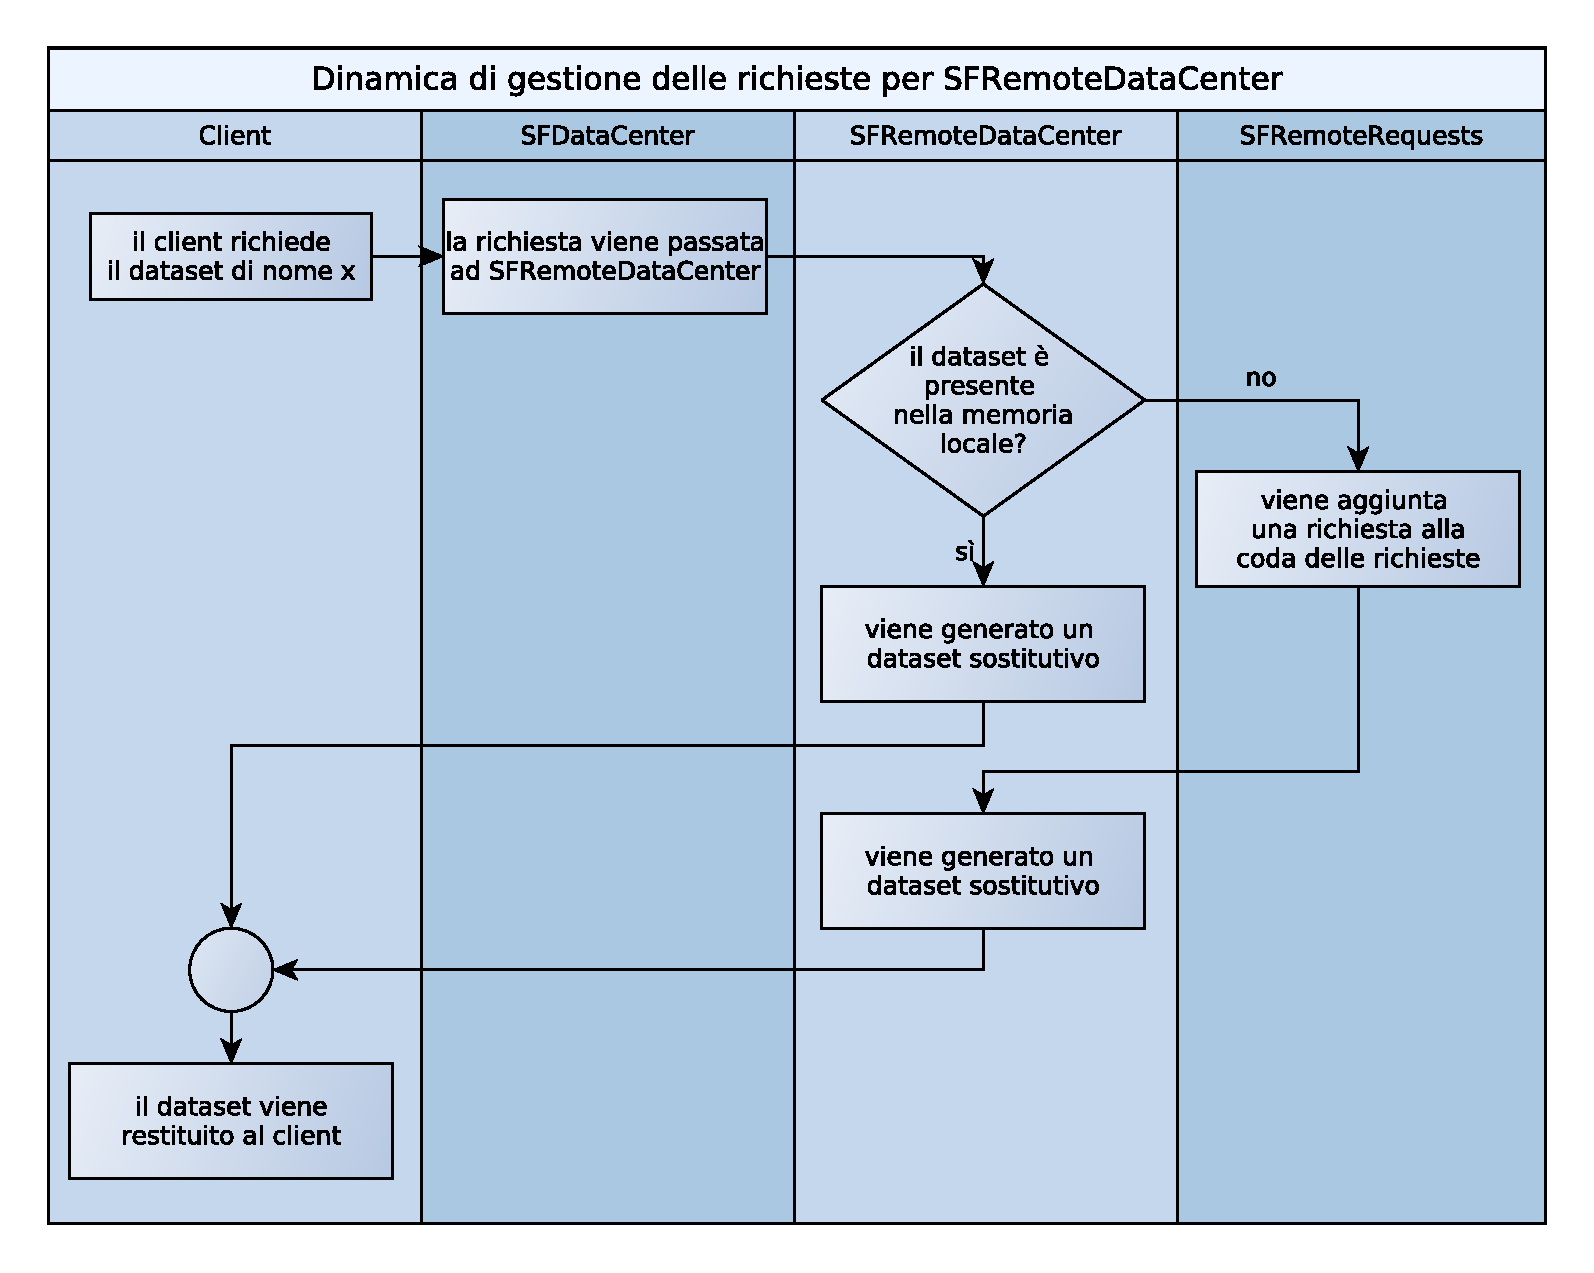
\includegraphics[width=\textwidth]{Immagini/DinamicaSFRemoteDataCenter}
\caption{Lo schema mostra la sequenza di eventi dovuti ad una richiesta a SFDataCenter che utilizza un SFRemoteDataCenter come implementazione interna.\label{f:dinamicasfremotedatacenter}} 
\end{center} 
\end{figure}

Questo modulo raggruppa una serie di classi pensate per essere una estensione del framework e per essere utilizzate principalmente all'interno di una applicazione client.
La sua funzione principale consiste nel fornire uno strato di comunicazione tra l'astrazione del reperimento dati fornita dal framework e il meccanismo di effettivo reperimento dei dati.

La classe chiave del modulo \`e \texttt{SFRemoteDataCenter}: questa \`e una classe di implementazione utilizzabile nel \textit{Bridge} realizzato da \texttt{SFDataCenter}\footnote{Per la classe \texttt{SFDataCenter} si rimanda al paragrafo \ref{sub:sfdatacenter} mentre per il pattern \textit{Bridge} al paragrafo \ref{sub:bridge}.}.
Dallo schema in figura \ref{f:dinamicasfremotedatacenter} osserviamo che le richieste di Dataset effettuate al DataCenter vengono passate a questa classe che le esamina verificando che il dato richiesto sia presente nella libreria dell'applicazione. Se il Dataset non \`e presente viene generata una richiesta e aggiunta ad un buffer di richieste di nome SFRemoteRequests, successivamente al richiedente \`e restituito un Dataset sostitutivo temporaneo scelto opportunamente. Il buffer, che supporta la sincronizzazione, pu\`o contemporaneamente essere utilizzato da un modulo esterno in grado di effettuare l'effettivo reperimento dei dati.
Il meccanismo dei Dataset sostitutivi viene descritto esaustivamente nella sezione \ref{sec:dataset_sost}.

% TODO: decidere se i 2 package aggiuntivi andrebbero inseriti nel modulo
Il modulo \`e composto dai package \texttt{shadow.system.data.remote.wip}, \texttt{shadow.system.data.object.wip} e \texttt{shadow.renderer.viewer.wip}.

\subsection{Client}
\label{sub:clientmodule}
Questo modulo raggruppa delle componenti generiche che possono essere utilizzate all'interno di una qualsiasi applicazione client e che servono ad implementare l'effettivo reperimento dei dati. 
Esso si pone al di sotto del modulo \textbf{RemoteDataCenter Tool} ed utilizza il modulo \textbf{Base Communication} per la gestione del canale di comunicazione e la sua implementazione \`e pensata per il multi-threading.
Il meccanismo messo a disposizione \`e mostrato nella figura \ref{f:dinamicaclient}, in esso un thread \texttt{RemoteDataCenterRequestsCreationTask} viene risvegliato periodicamente e controlla che non vi siano richieste pendenti nel buffer delle richieste. Se il buffer non \`e vuoto viene allora allocano un nuovo thread di tipo \texttt{RemoteDataCenterRequestTask} e mentre il precedente viene nuovamente sospeso questo effettua le richieste al server. Quando il secondo thread termina la comunicazione chiede al buffer di generare un update a tutti i client che avevano richiesto i dati reperiti e successivamente si chiude.


\begin{figure}
\begin{center}
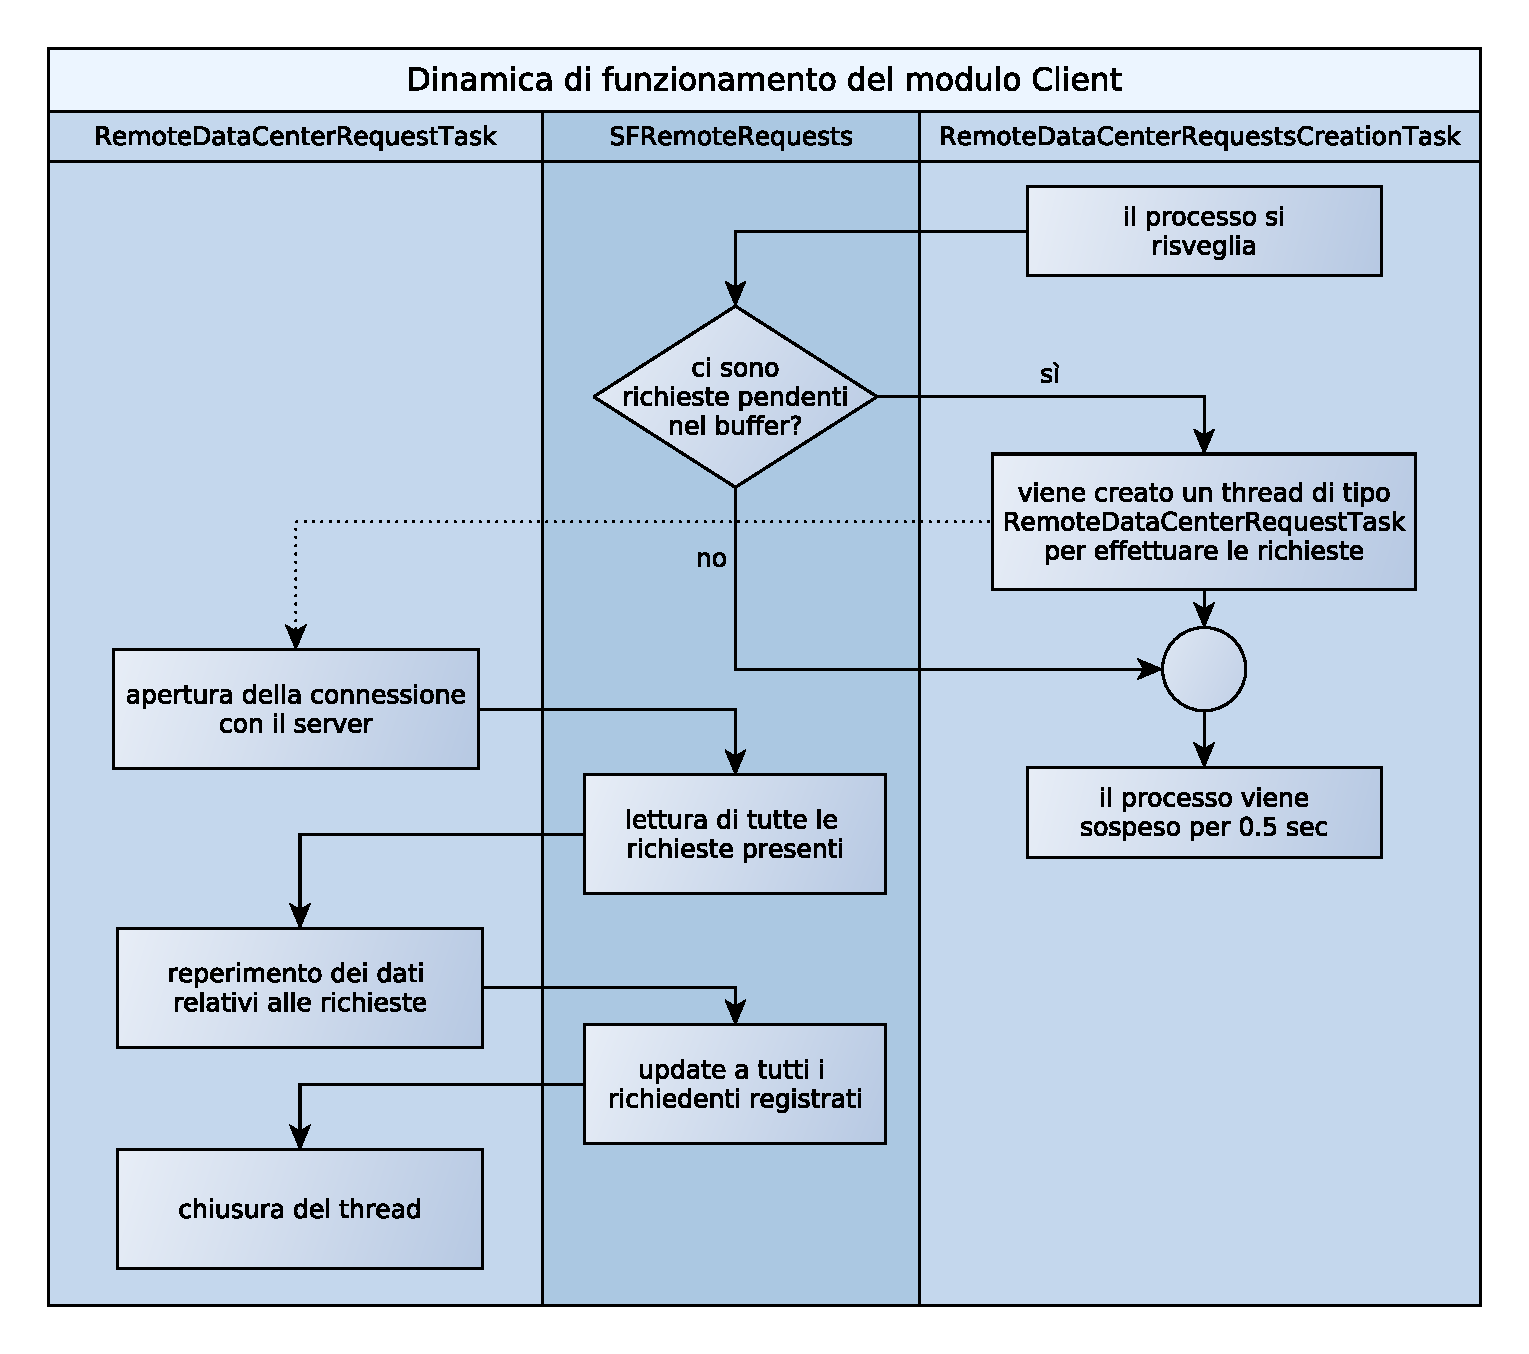
\includegraphics[width=\textwidth]{Immagini/DinamicaClient}
\caption{Dinamica del modulo client. Nello schema viene messa in evidenza la sostanziale indipendenza dei thread \texttt{RemoteDataCenterRequestsCreationTask} e \texttt{RemoteDataCenterRequestTask}, infatti a parte il fatto che i thread del secondo tipo sono creati dal primo non vi sono comunicazioni dirette tra i due.\label{f:dinamicaclient}} 
\end{center} 
\end{figure}


Il package che compone questo modulo \`e \texttt{sfrc.application.client}.

\subsection{Server}
\label{sub:servermodule}
Similmente al modulo per le componenti client, in questo vengono raggruppate delle componenti generiche utili alla realizzazione di una applicazione server. Queste componenti si pongono da tramite tra l'applicazione e il modulo di \textbf{Base Communication} tramite cui realizzano l'effetivo trasferimento dei Dataset verso il client connesso.
Anche in questo caso l'implementazione \`e pensata per il funzionamento multi-thread in parallelo con l'applicazione principale che pu\`o cos{\`\i} gestire pi\`u client connessi contemporaneamente ed eseguire altre operazioni.
Vengono fornite infine anche delle interfacce utili per effettuare l'inizializzazione dei dati e per configurare il protocollo di comunicazione.

Il modulo \`e composto dal package \texttt{sfrc.application.server}

\section{Dataset sostitutivi}
\label{sec:dataset_sost}
Per evitare che, in seguito alla richiesta di un Dataset non presente nella libreria locale di un'applicazione, i moduli richiedenti rimanessero in attesa dei dati bloccando di fatto l'esecuzione, \`e stato deciso di realizzare un meccanismo di sostituzione dei Dataset con successivo update delle richieste.
Successivamente ad una richiesta il RemoteDataCenter restituisce, attraverso la callback del richiedente, un Dataset sostitutivo temporaneo di tipo compatibile a quello richiesto.
Contemporaneamente viene generata una richiesta remota che attende di essere evasa. Quando i dati effettivi arrivano dalla rete viene eseguito un update del dato richiamando nuovamente la callback del richiedente.
Dato che pi\`u moduli dell'applicazione potrebbero fare richiesta dello stesso Dataset, tutte le callback dei richiedenti vengono memorizzate e, al momento dell'update, richiamate in successione.
% TODO: decidere se parlare dell'Updater
Per permettere il funzionamento di questo automatismo si \`e resa necessaria la realizzazione di un nuovo tipo di Dataset, l'SFDatasetReplacement, e di una libreria di Dataset sostitutivi.

Utilizzato all'interno di una ObjectsLibrary un DatasetReplacement permette di realizzare una lista di sostituzione che associa il nome di un Dataset "Alfa" richiesto, a quello di un Dataset sostitutivo di default "Beta" e ad un timestamp.
L'associazione tra nomi viene usata per una ricerca diretta del dato sostitutivo da utilizzare, mentre il timestamp \`e stato introdotto per lo sviluppo futuro di logiche di aggiornamento della lista di sostituzione.
Le liste di sostituzione sono state inoltre rese configurabili attraverso file XML leggibili dal decoder interno del framework.
% TODO: parlare del tool di generazione automatico?

La libreria dei Dataset di default \`e stata invece realizzata progressivamente durante l'implementazione dei test, quando si rendeva necessaria la costruzione di un Dataset specifico dato che quelli gi\`a realizzati erano di tipo incompatibile.
% TODO: specificare cosa si intende per tipo incompatibile

L'utilizzo di questo meccanismo richiede necessariamente una fase di inizializzazione in cui viene fatto il download o il caricamento da disco locale della lista di sostituzione e della libreria dei Dataset di default. Avendo la possibilit\`a di estendere il protocollo di comunicazione in modo da rendere espandibili queste due librerie durante l'esecuzione, \`e possibile mantenere la loro dimensione iniziale contenuta.

\section{Infrastruttura di rete} 
\label{sec:rete}
Date le specifiche iniziali esposte nel capitolo \ref{ch:introduzione}, una parte fondamentale del progetto \`e stata decidere quale infrastruttura per la comunicazione di rete sfruttare per poter utilizzare e testare il modulo \textbf{RemoteDataCenter Tool}, che si occupa della gestione delle richieste di Dataset.

%%%%%%%%%%%%%%%%%%%%%%%%%%%%%%%%%%%%%%%%%%%%%%%%%%%%%%%%%%%%%%%%%%

Se da lato client \`e ovvia la necessit\`a di sviluppare uno strato dell'applicazione che si occupa della comunicazione di rete, da lato server si sono presentate diverse possibilit\`a: 
%%%%%%%%%%%%%%%%%%%%%%%%%%%%%%%%%%%%%%%%%%%%%%%%%%%%%%%%%%%%%%%%%%

\begin{enumerate}
	\item  utilizzare un file server che permettesse semplicemente di accedere ai file contenti i dati tramite la rete;
	\item  utilizzare un application server java, come Tomcat o Glassfish, a cui un'applicazione client potesse connettersi e che attraverso l'esecuzione di servlet realizzasse il trasferimento dei dati da server a client;
	\item  utilizzare un'applicazione server ad-hoc appositamente sviluppata;
\end{enumerate}

La prima soluzione \`e probabilmente la pi\`u semplice, ma la meno flessibile dato che consente solo di un accesso diretto ai file di descrizione dei dati senza alcuna possibilit\`a di un'elaborazione lato server e spostando tutto il peso di un'eventuale interazione tra client direttamente su quest'ultimi.

La seconda soluzione offre pi\`u possibilit\`a e flessibilit\`a rispetto alla prima: l'utilizzo di un application server java mette a disposizione una piattaforma che consente una pre-elaborazione dei dati lato server e che possiede direttamente una serie di componenti per la gestione di compiti complessi legati alle sessioni degli utenti, come ad esempio l'autenticazione e la sicurezza. Nonostante i pregi, questo tipo di soluzione possiede anche lati negativi: gli application server generici non sono sviluppati per questo tipo di applicazioni e non era garantita una flessibilit\`a sufficiente per cui all'aumentare della complessit\`a del progetto e delle sue esigenze non fosse necessario abbandonare l'architettura. 

La terza soluzione \`e sicuramente la pi\`u flessibile ed estendibile dato che, se necessario, consente di modificare direttamente il server per adattarsi alle esigenze dell'applicazione. Lo svantaggio \`e la necessit\`a di dover implementare da zero tutte quelle funzionalit\`a non solo di comunicazione, ma anche di autenticazione o di sicurezza che una soluzione gi\`a pronta potrebbe possedere nativamente.

Nella scelta tra le tre soluzioni hanno pesato prevalentemente la volont\`a di realizzare un'architettura funzionante con la scrittura di meno codice possibile e quella di mantenere una bassa complessit\`a iniziale che non penalizzasse per\`o un'estensione futura delle funzionalit\`a. In quest'ottica la prima soluzione \`e stata anche la prima ad essere scartata, perch\'e sebbene garantisse un tempo di messa in opera molto basso non consente un'estensione di funzionalit\`a. 

La scelta finale \`e ricaduta sulla terza soluzione che pur costringendo a rinunciare alle funzionalit\`a avanzate della seconda, elimina difficolt\`a e tempistiche di una installazione e configurazione dell'application server. Inoltre, limitando inizialmente lo sviluppo a funzionalit\`a di base, \`e possibile limitare la complessit\`a del codice ad un livello non molto pi\`u elevato rispetto alla seconda soluzione.

\subsection{Protocollo di comunicazione}
\label{sub:comprotocol}
Una volta stabilito di utilizzare un server sviluppato appositamente \`e stato necessario stabilire le modalit\`a di comunicazione tra client e server. 

La comunicazione tra le applicazioni viene effettuata attraverso un protocollo basato su messaggi testuali che si colloca idealmente a livello di Sessione nel modello ISO/OSI \cite{book:computernetworking} mentre a livello inferiore viene utilizzato il protocollo TCP/IP.
L'utilizzo del TCP in quanto protocollo confermato \`e giustificato in quanto consente di garantire l'arrivo dei messaggi di comunicazione. Questi messaggi sono principalmente dedicati allo scambio dei dati grafici, per cui la garanzia di arrivo e l'integrit\`a dei dati sono prioritarie rispetto alle prestazioni.

% TODO: sistemare

I messaggi di comunicazione finora previsti sono strutturati secondo la seguente forma:
\begin{verbatim}
     etichetta_messaggio[:dati:opzionali:...]
\end{verbatim}
in cui \texttt{etichetta\_messaggio} identifica il tipo di messaggio, mentre i dati opzionali dipendono dal messaggio stesso e sono divisi dall'etichetta e tra loro dal carattere `` : ''.

Questi messaggi sono utilizzati all'interno di un preciso schema di interazione tra client e server di cui possiamo vedere un esempio nella figura \ref{f:clientserverinteraction}, da notare che la numerazione dei nodi rappresenta la sequenza temporale dello scambio di messaggi. Lo schema presentato mostra che, quando la coda delle richieste non \`e vuota, il client apre una connessione con il server ed invia un messaggio di tipo \textbf{request} in cui sono elencati i nomi dei Dataset di cui ha bisogno. Il server a questo punto genera una sequenza di risposte attraverso cui invia, se possibile, i dati richiesti. Al termine della sequenza invia un messaggio di tipo \textbf{reply-end} a cui il client risponde con un messaggio \textbf{closing} per terminare la connnessione.

\begin{figure}
\begin{center}
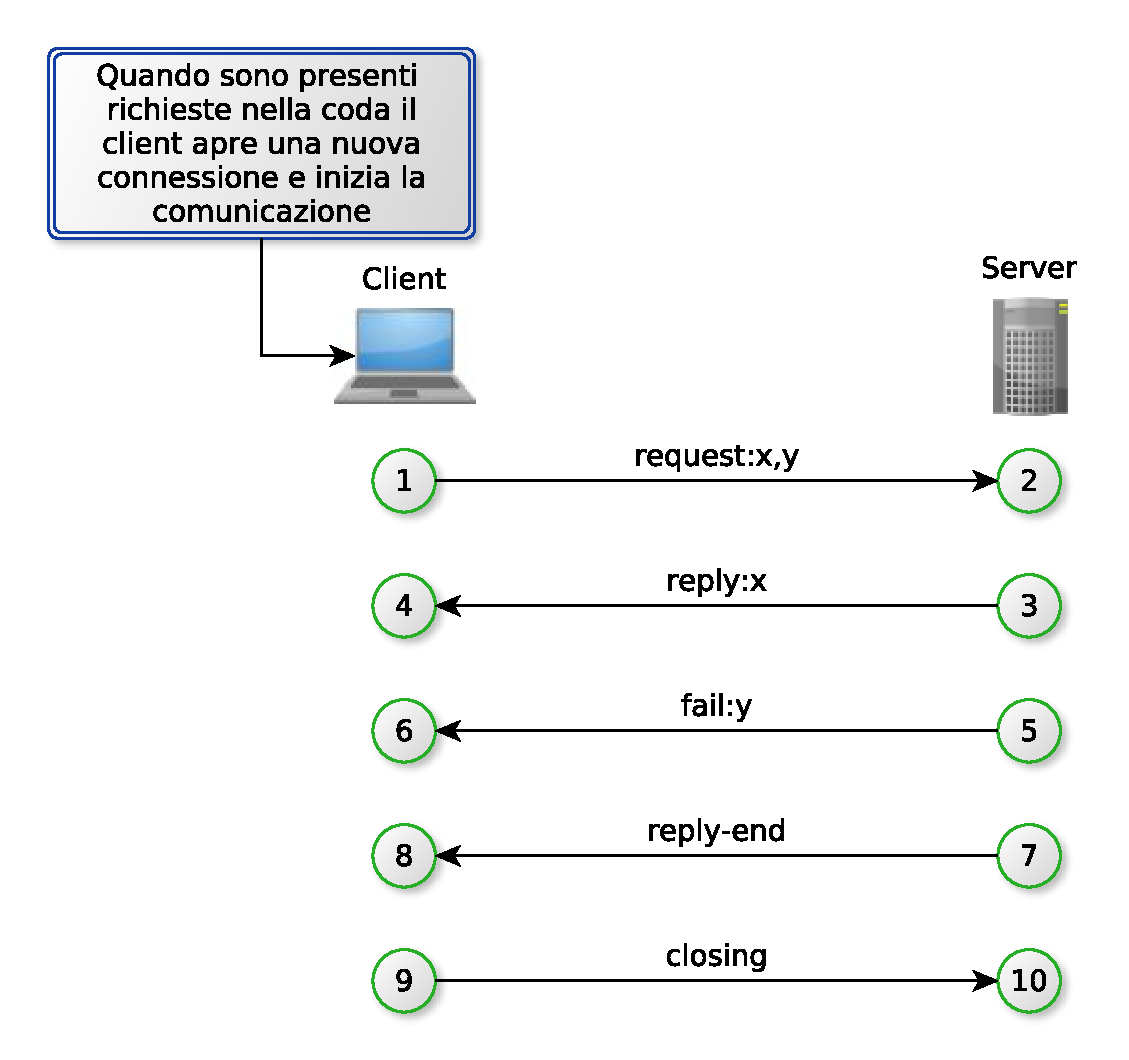
\includegraphics[width=10cm]{Immagini/InterazioniClientServer}
\caption{Esempio dello schema implementato per l'interazione tra client e server.\label{f:clientserverinteraction}} 
\end{center} 
\end{figure}

La gestione della comunicazione e dello schema di interazione viene effettuata tramite una macchina a stati specifica per client e server, le quali si occupano di leggere ed effettuare l'analisi logico-sintattica dei messaggi generando le eventuali risposte o semplicemente modificando lo stato interno della macchina stessa.

\begin{figure}
\begin{center}
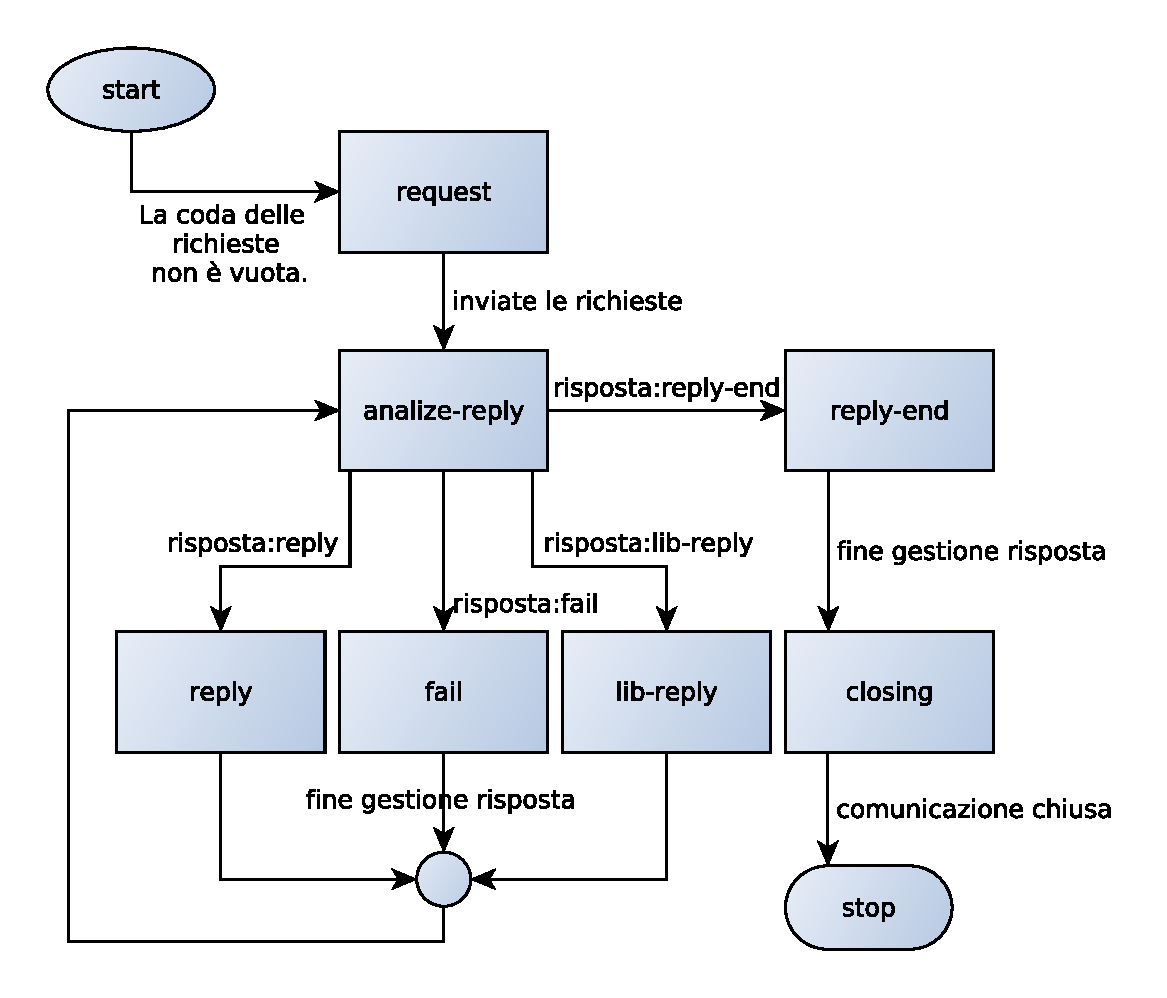
\includegraphics[width=11cm]{Immagini/StateMachineClient}
\caption{Diagramma a stati per la gestione della comunicazione delle richieste da parte del client.\label{f:stateclient}} 
\end{center} 
\end{figure}

Usare messaggi testuali per la comunicazione consente di semplificarne la gestione e rende possibile espandere il linguaggio semplicemente utilizzando nuove etichette, consentire tutto ci\`o ha per\`o reso necessario strutturare l'implementazione delle macchine a stati in modo che fossero altrettanto espandibili. Per far questo \`e stato preso come modello il pattern \textit{State}, descritto al paragrafo \ref{sub:state}, e la logica di ogni stato \`e stata incapsulata in un oggetto differente. Questo consente di espandere la macchina a stati semplicemente definendo nuovi oggetti i quali sono totalmente indipendenti dagli altri.

% TODO: rimandare alla classe protocol per la mappa del protocollo


I messaggi attualmente implementati sono:





\section{I Package java} 
\label{sec:sfrc_packages}
La classi che compongono il progetto sono suddivise in una serie di package. % TODO: decidere se la prossima frase va bene
Alcuni di questi sono pensati per rappresentare una possibile estensione a quelli forniti dal framework stesso e ne riproducono la struttura e le convenzioni sui nomi, gli altri sono librerie che affiancano il framework nella costruzione dell'applicazione.

